\chapter{Direct Dialling}
\label{ch:DirectDialling}

\begin{figure}[t]
  \begin{subfigure}{0.52\textwidth}
    \includegraphics{figures/recursive}
    \caption{}
    \label{fig:recursive}
  \end{subfigure}
  \begin{subfigure}{0.48\textwidth}
    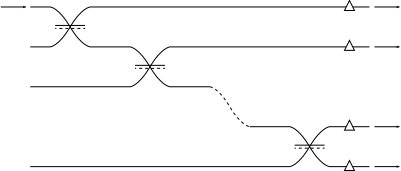
\includegraphics{figures/cascade}
    \caption{}
    \label{fig:cascade}
  \end{subfigure}
  \caption[Recursive decomposition of a unitary]
    {Recursive decomposition of a unitary. \ref{fig:recursive} shows an
    \(m \by m\) unitary as a product of \(m\) unitary transformations
    \(\mat{R}_{i}\), each acting on a successively larger subspace.
    \ref{fig:cascade} expands one of the \(\mat{R}_{i}\) unitaries in terms of
    a cascade of beamsplitters and phase shifts. The connection between the
    \emph{Cartesian} basis, \(\vec{x}\) and the \emph{physical} basis,
    \(\vec{r}\) is illustrated by the labels on \ref{fig:cascade}.}
  \label{fig:reck}
\end{figure}

\begin{figure}[t]
  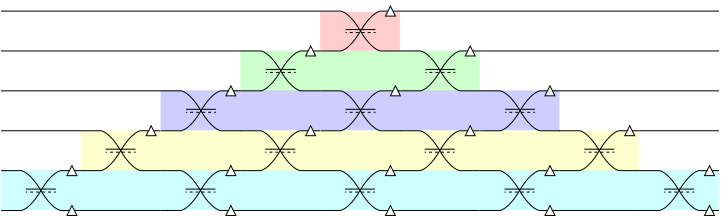
\includegraphics{figures/example}
  \caption[A $6 \by 6$ unitary, expressed in linear optics]
    {(a) A \(6 \by 6\) unitary, expressed in linear optics using a scheme
    similar to the one in \cite{reck}. (b) The \pdf{}s for
    beamsplitter reflectivities required to achieve Haar random unitaries.
    The reflectivities of beamsplitters on the
    bottom row can be chosen uniformly from the interval \(\left[ 0,1 \right)\),
    while those on higher rows are chosen from according to polynomials
    increasingly biased towards lower reflectivities. (c) A variable
    reflectivity beamsplitter can be implemented using a Mach Zehnder
    interferometer (MZI), composed of a phase shift, \(\theta\) between two
    50:50 beamsplitters (Hadamard operations). The phases may be chosen directly
    from the distributions shown, with increasing bias towards \(\theta=\pi\).
    (d) Finally, in integrated optics, variable refelectivity beamsplitters are
    implemented using an MZI composed of a phase shift, \(\xi\) between two
    50:50 directional couplers (symmetric Hadamards operations). The phases must
    then be chosen from the illustrated distributions, biased towards \(\xi=0\).
    Line colours in (b-d) correspond to shading in (a).}
  \label{fig:example}
\end{figure}

\section{Introduction}
\label{sec:DDIntro}
The development of the \bosonsampling{} problem \cite{bosonsampling} has
motivated fresh interest in studying \emph{random} unitaries that describe the
optical circuits acting on multiphoton states. Rapid developments in the field
of integrated optics with reconfigurable components facilitates the construction
of large-scale optical circuits capable of actively realising any unitary
operator. Combined with on-chip sources \cite{sources-josh} and detectors
\cite{detectors-munich, detectors-yale}, the scale of experimental
implementations of \bosonsampling{} \cite{bs-rome, bs-brisbane, bs-oxford,
bs-vienna} is likely to increase.

In linear optics, any unitary operator can be implemented as an array of
beamsplitters and phase shifters as shown in figure~\ref{fig:reck}. A similar
mathematical decomposition has been known for some time in the work of Hurwitz
\cite{hurwitz}, with the link to experimental components made more recently by
Reck et al. \cite{reck}. Here we present a simple procedure for choosing
a Haar random unitary on an optical circuit by choosing values of the physical
parameters independently from simple distributions. This procedure is useful in
applications such as \bosonsampling{} where we do not need to know the exact
unitary description of the circuit being implemented, but need a guarantee that
it is drawn from the correct distribution. While similar parameterisations exist
in the mathematical literature \cite{spengler2012, zy-jpa-27-4235}, the
relevance to linear optics is not widely appreciated. Further, we extend the
result to systems of qubits, by deriving a mapping between a linear-optical
circuit on \(m=2^{n}\) modes and a circuit operating on \(n\) qubits.

\section{A physically-motivated parameterization}
\label{sec:Parameterization}
Drawing a Haar random unitary is analogous to choosing a random number from a
uniform distribution in that it should be unbiased. The probability of drawing
a particular unitary matrix from some region in the space of unitaries should
be in direct proportion to the volume of the region as defined by the Haar
measure, which is the unique translation-invariant measure on the space of
unitaries. As argued in \cite{reffy}, if \(m\) vectors \(\left\{
v_{i} \right\} = \left\{ v_{1}, v_{2}, \cdots, v_{m} \right\}\) are successively
drawn from the unbiased distribution of unit vectors in the
\(\left(m-i\right)\)-dimensional subspace orthogonal to all previous vectors,
they form the columns of a Haar random unitary. The problem of choosing Haar
random unitaries thus reduces to the problem of drawing such a set of orthogonal
vectors.

We approach this problem by considering a general linear optical circuit, shown
in figure~\ref{fig:recursive}, which suggests a recursive strategy for
achieving the appropriate set of \(m\) vectors for a unitary operation on \(m\)
modes. Each block labelled \(\mat{R}_{n}\) takes
as input the basis state \( \ket{m-n}\) and performs a unitary operation to
produce the \(n\)-dimensional vector \(\ket{v_n}\). Orthogonality is preserved
as this vector is transformed by all subsequent \(\mat{R}_{i}\). Further, if the
vector \(\ket{v_{n}}\) is chosen from the unbiased distribution of unit vectors
in \(n\) dimensions, the property of left invariance ensures that it does not
become biased by the operation of the subsequent \(\mat{R}_{i}\).

The next consideration is therefore how to choose appropriate vectors, i.e.\
unbiased unit vectors, in \(n\) dimensions. Figure~\ref{fig:cascade} expands one
of the \(\mat{R}_{i}\) in terms of linear optical components, and we proceed
from here. Consider the complex Gaussian vector in \(n\) dimensions:
\begin{equation}
  \ket{\vec{v}_{n}} = \sum_{i=0}^{n-1} z_{i} \ket{i} = \sum_{i=0}^{n-1} \tau_{i}
  e^{i \alpha_{i}} \ket{i}
\end{equation}
where the \(z_i\) are i.i.d. Gaussian complex numbers, \( \prob{P}_{z} \of{z}
\propto \exp \left( -\abs{z}^2 \right) \). Because of their independence, the
probability density function (\pdf{}) for \(\vec{v}_n\) is the product of the
\pdf{}s for the elements and depends only on the magnitude of the vector. Let
\(x_i = \abs{z_i}^2 \), then:
\begin{equation}
  \label{eq:vec}
  \prob{P}_{\vec{v}_n} = e^{ -\left(x_0 + x_1 + \dots + x_{n-1} \right)} = e^{
  -\abs{\vec{v}_n}^2}
\end{equation}
Now consider the change of variables from this basis~\(\vec{x}\), which we call
the Cartesian basis, to a new basis,~\(\vec{r}\):
\begin{align}
  r_0 &= \sum_{k=0}^{n-1} x_k \\
  r_i &= \frac{x_{i-1}}{\sum_{k=i}^{n-1} x_k} & \left( 0 < i \leq n-1 \right) \\
  \phi_i &= \alpha_{i}
\end{align}
We refer to \(\vec{r}\) as the physical basis because the variables
correspond directly to components in a physical realisation of the vector in
linear optics. In particular, \(r_0\) is the power of the input and the other
\(r_i\) are reflectivities of beamsplitters. The relationship between
\(\vec{x}\), \(\vec{r}\) and the physical system is shown in
figure~\ref{fig:reck}.

In order for this parameterisation to be useful, we must show that the \pdf{}
for the vector \(\vec{v}_n\) is separable in the physical basis so that the
experimental parameters can be chosen independently. We also need to derive the
form of the marginal distributions for the \(r_i\) and \(\phi_{i}\). These will
be the distributions from which experimental parameters must be chosen to
obtain a Haar unitary. Since there is no functional dependence on the
\(\alpha_{i}\) parameters in equation~\ref{eq:vec} and there is a one-to-one
mapping \(\alpha_{i} \rightarrow \phi_{i}\), these phases can be chosen
uniformly and independently from the interval \(\left[0,2\pi\right)\)

Finding the \pdf{}s for the beamsplitter reflectivities requires a more careful
change in bases, using the Jacobian:
\begin{equation}
  \prob{P}_{\vec{v}_n} \of{\vec{r}} = \prob{P}_{\vec{v}_n} \of{\vec{x}}
  \abs{\det \mat{J} \of{\vec{x}, \vec{r}}}
\end{equation}
where
\begin{equation}
  \mat{J}_{i,j} \of{\vec{x}, \vec{r}} = \frac{\partial x_{i}}{\partial r_j}
\end{equation}
Equation~\ref{eq:vec} is expressed in the \(\vec{r}\) basis simply as \(\exp
\of{-r_0}\), so is trivially separable. We now consider the Jacobian
determinant, which is described by the four cases:
\begin{align}
  \label{eq:firstcolumn}
  \mat{J}_{i,j} &= r_{i+1} \prod_{k=1}^{i} \left( 1-r_k \right) && j=0 \\
  \mat{J}_{i,j} &= \frac{-r_0 r_{i+1}}{1-r_{j}} \prod_{k=1}^{i} \left( 1-r_k
    \right) && 0< j \leq i\\
  \label{eq:diagonal}
  \mat{J}_{i,j} &= r_0 \prod_{k=1}^{i} \left( 1-r_k \right) && j = i+1 \\
  \mat{J}_{i,j} &= 0 && j>i+1
\end{align}
(where the variable \(r_{n}=1\) has been introduced for convenience)

A matrix of this form (lower Hessenberg) can always be transformed into a
lower triangular matrix---for which the determinant is simply the product of the
diagonal elements---by column operations, which do not change the absolute value
of the determinant. The first step is to perform a set of operations on the
\(j=0\) column, \(\vec{c}_{0}\) that set the upper \(n-1\) terms to zero, as
follows:
\begin{equation}
  \label{eq:columns}
  \vec{c}_{0}^{\left( k \right)} = \vec{c}_{0}^{\left( k-1 \right)} -
  \vec{c}_{k} \frac{\mat{J}_{k-1,0}^{\left( k-1 \right)}}{\mat{J}_{k-1,k}}
\end{equation}
where \(k\) runs from \(1\) to \(m-1\). None of these operations changes the
value of the determinant, and we now show that after the procedure is complete
the element \(\mat{J}_{0,n-1}=1\).

The \(k^{\text{th}}\) operation in equation~\ref{eq:columns} is designed to set
\(\mat{J}_{k-1,0}^{k}=0\), by subtracting column \(\vec{c}_{k}\) multiplied by an appropriate scalar. The effect on all
the other elements of \(\vec{c}_{0}\) is to remove the dependence on \(r_{k}\),
which we can prove inductively.

Suppose that after \(k\) such operations, the upper \(k\) elements of
\(\vec{c}_{0}\) have been set to zero and the remaining elements have no
dependence on \(r_{l}\) for \(0 \leq l \leq k\). We can express the elements of
\(\vec{c}_{0}^{\left(k\right)}\) as:
\begin{equation}
  \label{eq:koperations}
  \mat{J}_{i,0}^{\left(k\right)} = \left\{ \begin{array}{lcl}
    r_{i+1} \displaystyle \prod_{l=k+1}^{i} \left( 1-r_{l} \right) & , &
      i \geq k \\
    0 & , & i < k
  \end{array} \right.
\end{equation}
The base case is \(k=0\), where the expression in equation~\ref{eq:firstcolumn}
is recovered. We now perform the \(\left(k+1\right)^{
\text{th}}\) operation on all non-zero rows (i.e.\ \(i \geq k+1\)):
\begin{align}
  \mat{J}_{i,0}^{\left(k+1\right)} &= \mat{J}_{i,0}^{\left(k\right)} - 
    \frac{\mat{J}_{k,0}^{\left(k\right)}}{\mat{J}_{k,k+1}} \mat{J}_{i,k+1} \\
  &= r_{i+1}\prod_{l=k+1}^{i} \left( 1-r_{l} \right) + \frac{\displaystyle
    r_{k+1} \prod_{
    l=k+1}^{k} \left( 1-r_{l} \right) }{\displaystyle r_{0} \prod_{l=1}^{k}
    \left( 1-r_{l} \right) } \frac{ r_{0} r_{i+1} }{ \left( 1-r_{k+1} \right) }
    \prod_{ l=1 }^{i} \left( 1-r_{l} \right) \\
  &= r_{i+1} \prod_{l=k+1}^{i} \left( 1-r_{l} \right) + \frac{ r_{k+1} r_{i+1}
    }{ \left( 1-r_{k+1} \right) } \prod_{l=k+1}^{i} \left( 1-r_{l} \right) \\
  &= r_{i+1} \left( 1-r_{k+1} \right) \prod_{l=k+2}^{i} \left( 1-r_{l} \right)
    + r_{i+1} r_{k+1} \prod_{l=k+2}^{i} \left( 1-r_{l} \right) \\
  &= r_{i+1} \left( 1-r_{k+1}+r_{k+1} \right) \prod_{l=k+2}^{i} \left( 1-r_{l}
    \right) \\
  &= r_{i+1} \prod_{l=k+2}^{i} \left( 1-r_{l} \right)
\end{align}
We recover the expression in~\ref{eq:koperations}, thus proving the result.
After \(n-1\) iterations, we find that \(\mat{J}_{n-1,0}^{\left(n-1\right)}=
r_{n}=1\), recalling that \(r_{n}=1\) was a variable introduced for convenience.

We can then place the column \(\vec{c}_{0}\) as the rightmost column, at which
point the matrix is lower triangular and we can compute the determinant by
multiplying the diagonal elements of the matrix. Since the shift, these are the
elements given by equation~\ref{eq:diagonal}.
\begin{equation}
  \det \mat{J} \of{ \vec{x}, \vec{r} } = \prod_{i=1}^{n-1} \mat{J}_{i,i}
\end{equation}
and the explicit form of the \pdf{} in the \(\vec{r}\) basis is
\begin{equation}
  \prob{P}_{\vec{v}_n} \of{ \vec{r} } = e^{-r_0} r_0^{n-1} \prod_{k=1}^{n-2}
  \left( 1-r_k \right)^{n-k-1}
\end{equation}
which is manifestly separable.

It can be verified by explicit integration that this expression is appropriately
normalised. Since the \pdf{} is separable in this basis, the variables \( r_i
\) are independent, and can be chosen according to their marginal distributions,
\begin{align}
  \prob{P}_{r_{i}} \of{r} = \left( n-i \right) \left( 1-r \right)^{n-i-1} &&
  1 \leq i < n
\end{align}
We now integrate over \(r_{0}\) to obtain a compact form for the \pdf{} of
\(n\)-dimensional \emph{unit} vectors,
\begin{equation}
  \prob{P}_{ \vec{u}_n } = \left( n-1 \right)! \prod_{k=1}^{n-1} \left( 1-r_k
  \right)^{n-k-1}
\end{equation}
and express the \pdf{} for the full circuit of beamsplitters,
\(\prob{P}_{\vec{C}}\) as the product of the \pdf{}s for the diagonal arrays of
beamsplitters:
\begin{equation}
  \prob{P}_{\vec{C}} = \prod_{j=1}^{n} \left[ \left( j-1 \right)!
  \prod_{k=1}^{j-1} \left( 1-r_{j,k} \right)^{j-k-1} \right]
\end{equation}
where \( r_{j,k} \) is the reflectivity of the \( k^{\text{th}} \) beamsplitter
in the \( j^{\text{th}} \) rotation, \( \mat{R}_j \).

In practical terms, an optical circuit conforming to a Haar unitary can be
fabricated with reflectivities and phase shifts chosen from the correct
distributions, as described here. A \( 6 \by 6 \) example is illustrated in
figure~\ref{fig:example}.

\section{Extension to qubits}
\label{sec:Qubits}
We now extend the result to the case of a unitary operating on qubits by
demonstrating a mapping between a unitary operation on \(m=2^{n}\) optical
modes and the same unitary operation on \(n\) qubits. The gates that we use to
construct the mapping are the Hadamard gate, the CNOT gate (generalised to
include multiple control) and variable phase gates, which implement a general
phase rotation on a qubit, as follows:
\begin{align}
  \Phi &= \begin{pmatrix}
    1 & 0 \\
    0 & e^{i\phi}
  \end{pmatrix} &
  \overline{\Phi} &= \begin{pmatrix}
    e^{i\phi} & 0 \\
    0 & 1
  \end{pmatrix}
\end{align}
Figure~\ref{fig:qubits} illustrates how this mapping is constructed, including
an explicit example of 2 qubits or 4 optical modes. Each optical phase is
implemented by a \(\Phi\) gate, and each beamsplitter is implemented by a
\(\Phi\) gate between two Hadamards (\(\mathrm{H \cdot \Phi \cdot H}\)),
effectively implementing a Mach Zehnder interferometer (MZI).

The existence of this mapping means that we can directly apply the results
described above to the implementation of Haar unitaries in systems of qubits,
with the only difference being the description of a varible reflectivity element
in terms of the internal phase \(\theta\) in an MZI. A further change of
variables, \(r = \sin^{2} \of{\theta} \) is required, and the appropriate
\pdf{}s for these elements are then:
\begin{equation}
  \prob{P}_{\theta_{i}} \of{ \theta } = \left( n-i \right) \cos \of{
  \frac{\theta}{2} } \sin \of{ \frac{\theta}{2} }^{2 \left(n-i\right) -1}
\end{equation}
These distributions are illustrated in figure~\ref{fig:example} alongside those
for reflectivities.

\begin{figure}[p]
  \includegraphics{figures/qubits}
  \caption[Mapping between a linear optical circuit and a unitary operating on
    qubits]
    {Mapping between a linear optical circuit and a unitary operating on
    qubits. A shorthand is used in the qubit picture for multiple control of
    operations. A solid circle on a qubit indicates that the operation is
    performed conditional on the `1' state of the control qubit, while an empty
    circle indicates controlling the operation on the `0' state. The gates
    labelled \(\Phi\) indicate performing a phase shift of \(\Phi\) radians on
    the `1' state of the target qubit and those labelled \(\overline{\Phi}\)
    perform a phase shift of \(\Phi\) radians on the `0' state of the target
    qubit. \\
    In (a) the 2-qubit (4 optical mode) unitary is drawn out explicitly.
    (b-d) correspond to the elementary operations for a 3 qubit (8 optical mode)
    unitary. (b) shows how a phase shift on any of the modes can be
    implemented. \\
    The beamsplitters in (c) are in the `even' positions, meaning that they
    operate on pairs of modes that differ only in the state of the third (final)
    qubit. These can be implemented in the qubit picture by controlled phases
    between Hadamard gates. \\
    (d) deals with the `odd' beamsplitters, which act on
    pairs of modes that may differ in the state of more than one qubit. In this
    case, a series of multiply-controlled NOT gates are required as well as the
    Hadamards. In both (c) and (d) any subset of the beamsplitters may be
    implemented on qubits by simply omitting controlled phases where
    appropriate. \\
    The parameters in the qubit picture are the phases in the
    controlled-\(\Phi\)
    gates. There is a one-to-one mapping between these phases and the
    beamsplitters in a linear optical circuit so in order to
    choose a Haar random unitary, we can use the distributions expressed in
    figure~\ref{fig:example}(d).}
  \label{fig:qubits}
\end{figure}
  
\section{Variable reflectivity beamsplitters}
\label{sec:integrated}

The discussion of linear optical circuits in linear optics makes use of a
variable reflectivity beamsplitter as a primitive component. In terms of the
power reflectivity, \(r\), the matrix describing this component is
\begin{equation}
  \mat{BS} \of{r} = \begin{pmatrix}
    \sqrt{r} & \sqrt{1-r} \\
    \sqrt{1-r} & -\sqrt{r}
  \end{pmatrix}
\end{equation}
In the qubit picture, we avoid implement a variable-reflectivity beamsplitter as
a variable phase shift, \(\theta\) between two Hadamard operations. The matrix
representation of this component is (down to global phase)
\begin{equation}
  \mat{MZI}_{\mat{H}} \of{\theta} = \begin{pmatrix}
    \cos \of{ \frac{\theta}{2} } & i \sin \of{ \frac{\theta}{2} } \\
    i \sin \of{ \frac{\theta}{2} } & \cos \of{ \frac{\theta}{2} }
  \end{pmatrix}
\end{equation}
We use the coordinate transformation \( r \rightarrow \cos \of{ ^{\theta}/_{2}}
\) to find the \pdf{}s in terms of this phase shift, rather than the
reflectivity.

An implementation in integrated optics would be similar, but instead of using
the Hadamard,
\begin{equation}
  \mat{H} = \frac{1}{\sqrt{2}} \begin{pmatrix}
    1 & 1 \\
    1 & -1
  \end{pmatrix}
\end{equation}
we use directional couplers, which implement the symmetric version
\begin{equation}
  \mat{DC} = \frac{1}{\sqrt{2}} \begin{pmatrix}
    1 & i \\
    i & 1
  \end{pmatrix}
\end{equation}

The resulting MZI is described in terms of its internal phase \(\xi\) (again,
down to a global phase) by the matrix
\begin{equation}
  \mat{MZI}_{\mat{DC}} \of{\xi} = \begin{pmatrix}
    \sin \of{ \frac{\xi}{2} } & \cos \of{ \frac{\xi}{2} } \\
    \cos \of{ \frac{\xi}{2} } & -\sin \of{ \frac{\xi}{2} }
  \end{pmatrix}
\end{equation}
The appropriate transformation between reflectivity and internal phase is now
\(r \rightarrow \sin \of{^{\xi}/_{2}} \), resulting in different \pdf{}s, which
are shown in figure~\ref{fig:example}d.

\section{Conclusions}
\label{sec:DDConclusions}
We have shown how to express the probability density function for Haar random
unitary matrices in terms of physically motivated parameters. The expression is
compact and non-redundant, whereas the equivalent in the Cartesian basis is a
lot more complicated. While the mathematics of this process has been known
for some time, the link to linear-optical components has not previously been
made clear, and the proof presented here in terms of a change of basis is much
simpler than that in \cite{spengler2010}. The formula in its general form
is applicable to \bosonsampling{}, where Haar unitaries are required, and is
extensible to systems of qubits so may find additional applications outside of
linear optics.
